\chapter{Marco teórico}
\label{capitulo3}
\lhead{Capítulo 3. \emph{Marco teórico}}

El presente capítulo tiene como intención exponer las bases teóricas necesarias para el desarrollo de este trabajo. Este capítulo se divide en cuatro secciones: la Sección \ref{sec:teo-uav} explica la teoría relacionada con el modelo de los vehículos aéreos no tripulados (UAV, del inglés \textit{unmanned aerial vehicle}), en particular, los UAV de cuatro rotores; la Sección \ref{sec:teo-stereo} describe el funcionamiento de los algoritmos utilizados para la obtención de mapas de profundidad a partir de un sistema de visión estereoscópica; la Sección \ref{sec:teo-neural} explica la teoría relacionada con las redes neuronales y Redes Neuronales Convolucionales (CNN, del inglés \textit{Convolutional Neural Networks}); finalmente, la Sección \ref{sec:teo-interprocess} describe el funcionamiento de los protocolos de comunicación entre procesos utilizados en este trabajo.

\section{Vehículos aéreos no tripulados de cuatro rotores}
\label{sec:teo-uav}

Un vehículo aéreo no tripulado de cuatro rotores, también llamado \textit{Quadrotor} UAV (abreviado QUAV a efectos de este trabajo) es una aeronave no tripulada propulsada por cuatro rotores que es controlada por un operador en tierra. Los QUAVs pertenecen a la familia de los drones y su principal característica es que la configuración de los cuatro rotores les permite rotar y elevarse independientemente mediante control de la velocidad de rotación de los rotores \cite{multidrone2017review}; el mismo mecanismo les permite moverse omni-direccionalmente, así como también flotar en sitio (del inglés \textit{hovering in place}). Debido a que su funcionamiento es enteramente dependiente del empuje producido los rotores, los QUAVs generalmente tienen un tiempo de vuelo máximo bastante reducido (menos de 30 minutos en promedio \cite{multidrone2017review}), pues baterías de alta capacidad de carga introducen peso en el sistema que puede afectar considerablemente la capacidad de vuelo del vehículo; sobre esta misma linea, el limite de masa de carga de estos vehículos es generalmente bastante pequeño. Estas características de los QUAVs hacen que su uso sea atractivo para aplicaciones donde la agilidad es un factor importante, siempre y cuando la capacidad de carga necesaria sea relativamente baja y tiempos de vuelo inferiores a 30 minutos sean aceptables \cite{multidrone2017review}. En el Capítulo \ref{capitulo2}, en la Figura \ref{fig:acsl-products} se muestra SOTEN, un QUAV diseñado por ACSL para aplicaciones de fotografía aérea (inspección, vigilancia, entre otras) y que sirve de plataforma física para el desarrolo del presente trabajo. Con la finalidad de comprender la estructura y condiciones de arquitectura de la plataforma física, a continuación se da una breve descripción de los componentes de un QUAV. 

\subsection{Componentes}

La configuración de componentes general de los QUAVs, si bien bastante amplia y llena de excepciones, cuando se remiten a los QUAVs comerciales, se puede englobar en: Un conjunto de sensores, que se utilizan principalmente para localizar el vehículo en el entorno; una unidad de control de vuelo (FCU, del inglés \textit{Flight Control Unit}), encargada de controlar la velocidad de rotación de los rotores; al menos una computadora a bordo (\textit{Onboard PC} en inglés), que se encarga de realizar el procesamiento necesario para llevar a cabo tareas de alto nivel, como la evasión de obstáculos y el mapeo del entorno; y una estación de control en tierra (GCS, del inglés \textit{Ground Control Station}) \cite{multidrone2017review}. 

\subsubsection*{Sensores}
\label{sec:QUAV-sensors}

Es de vital importancia que un QUAV tenga la capacidad de estimar su estado (orientación, altitud, posición y velocidad) utilizando solamente los componentes disponibles a bordo del vehículo. Para la estimación de orientación se utiliza una unidad de mediciones inerciales \cite{multidrone2017review} (IMU, del inglés \textit{Inertial Measurement Unit}) que se compone de un acelerómetro y giroscopio, ambos midiendo sus cantidades con respecto al marco de referencia del cuerpo del vehículo. Adicionalmente, también se puede utilizar un magnetómetro (brújula), para obtener la información de la orientación del vehículo con respecto al norte magnético del planeta tierra. Utilizando la información del IMU y del magnetómetro, el FCU puede estimar la orientación del cuerpo del vehículo con un nivel de precisión aceptable \cite{multidrone2017review}.

Para la estimación de posición y velocidad se puede emplear localización visual utilizando algoritmos de localización y mapeo con cámaras estereoscópicas o LiDAR \cite{multidrone2017review}. Estos algoritmos pueden llegar a tener limitaciones considerables cuando las condiciones de iluminación no son ideales y su rendimiento en entornos al aire libre es limitado debido a la uniformidad de las texturas del entorno \cite{multidrone2017review}. Alternativamente se puede utilizar GPS (del inglés \textit{Global Postionaing System}) para la localización a partir de señales de satélite \cite{multidrone2017review}; en este esquema la posición es estimada mediante triangulación entre el vehículo y un sistema de satélites, la velocidad es estimada utilizando el efecto \textit{doppler} y la altitud se estima utilizando un barómetro (sensor de presión atmosférica) o un sistema sonar \cite{multidrone2017review}. La localización por GPS es bastante efectiva para su uso en entornos al aire libre, pero no es posible utilizarlo en aplicaciones que naveguen en interiores debido al requerimiento de tener recepción de las señales de los satélites. Es común que un QUAV tenga acceso tanto a localización por visión como a localización por GPS, alternando entre ambas dependiendo de las condiciones de iluminación y recepción del satélite.

\subsubsection*{FCU}
\label{sec:QUAV-FCU}

Este componente maneja la estimación del estado del QUAV a partir de las señales de los sensores, así como el cálculo de las acciones de control para mantener estabilidad durante el vuelo. El FCU ofrece distintos modos de control, desde asistencia de orientación, asistencia en posición y asistencia de velocidad; todos estos con la finalidad de que controlar el QUAV en alto nivel sea una tarea más sencilla tanto para un operador como para otro algoritmo de alto nivel (como la evasión de obstáculos, el caso de este trabajo). 

\subsubsection*{Computadora a bordo}

Ejecuta los algoritmos de alto nivel que requieren más poder de cómputo para su procesamiento, tales como algoritmos de localización por visión, inferencia con redes neuronales, procesamiento y \textit{broadcasting} de imágenes, mapeo del entorno, entre otros. Algunas se equipan con unidades de procesamiento gráfico (GPU, del inglés \textit{Graphics Processing Unit}) que contribuyen en la aceleración de las operaciones de procesamiento distribuido o de inferencia de redes neuronales, en ambos casos utilizando tecnologías como CUDA (Arquitectura Unificada de Dispositivos de Cómputo, del inglés: \textit{Compute Unified Device Architecture}). La solución propuesta en el presente trabajo se implementa y ejecuta justamente dentro de la computadora a bordo del QUAV.

\subsubsection*{GCS}

Estación de control en el suelo, permite que el operador en suelo coordine las operaciones que hace el QUAV, en otras palabras, sirve de interfaz de alto nivel entre el operador y las funciones implementadas en el QUAV. Usualmente se utiliza para planificar vuelos autónomos, monitorizar el estado de los sensores, realizar \textit{streaming} de las imágenes de los sensores visuales del vehículo (cámaras), lanzar rutinas de control como aterrizaje o despegue automático, así como también instrucciones especificas de la aplicación (por ejemplo, entregar paquete para QUAV orientado a \textit{delivery}).

En la Figura \ref{fig:QUAV-components} se muestra el diagrama de comunicación general de los componentes de un QUAV, además de los componentes descritos anteriormente, se muestra la interacción con el radio control que es controlado por el operador, este además de encargarse de la transmisión de los comandos de operación vía señales de radio, se puede utilizar para operar el vehículo directamente o en conjunción con la GCS para orquestar operaciones complejas. 

\begin{figure}[H]
    \centering
    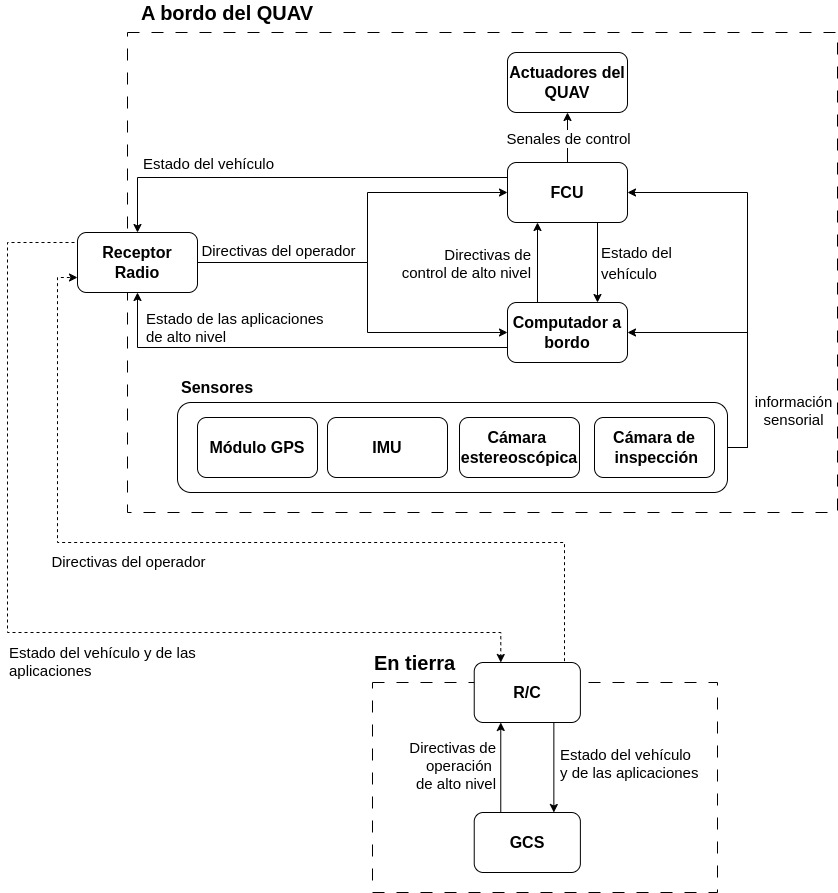
\includegraphics[scale=0.45]{partes/img/QUAV-components.jpg}
    \caption[Diagrama de comunicación general del los componentes de un QUAV.]{Diagrama de comunicación general del los componentes de un QUAV.} 
    \label{fig:QUAV-components}
\end{figure}

\subsection{Información relevante del modelo del QUAV}

En este trabajo no se hace una revisión completa del modelo cinemático y dinámico de un QUAV, sin embargo, es necesario discutir algunos conceptos que son utilizados en el desarrollo e implementación del algoritmo de evasión de obstáculos.

\subsubsection*{Sistemas de referencia}

Existen dos sistemas de referencia de interés para el manejo de QUAV: el sistema de referencia inercial \jim{E}, usualmente anclado a la superficie de la tierra; y el sistema de referencia del cuerpo del vehículo \jim{B}, que se encuentra anclado a centro del marco del QUAV. Tal como se aprecia en la Figura \ref{fig:QUAV-model}, la rotación del sistema del cuerpo \jim{B}, es representada por \jim{\phi,\theta,\psi} \cite{multidrone2015modeling}, donde: \jim{\phi} es denominado rolido \textit{roll} y representa la rotación con respecto al eje inercial \jim{x}; \jim{\theta} es denominado \textit{pitch} y representa la rotación con respecto al eje inercial \jim{y}; y \jim{\psi} es denominado \textit{yaw} y representa la rotación con respecto al eje inercial \jim{z}. Por convención, la velocidad lineal del vehículo \jim{V_B} se expresa en el sistema \jim{B}.

\begin{figure}[H]
    \centering
    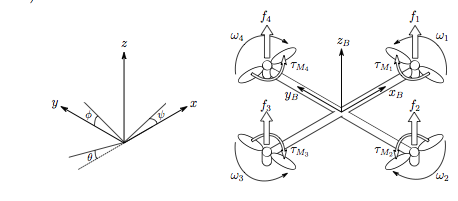
\includegraphics[scale=0.65]{partes/img/QUAV-model.png}
    \caption[Diagrama de un QUAV.]{Diagrama de un QUAV \cite{multidrone2015modeling}.} 
    \label{fig:QUAV-model}
\end{figure}

Es necesario establecer una transformación entre \jim{B} y \jim{E}, para ello podemos derivar una matriz de rotación a partir de rotaciones sucesivas dadas por \jim{\phi,\theta,\psi}, este tipo de transformación obtenida a partir de rotar \jim{\phi,\theta,\psi} se denomina transformación por ángulos de Euler \cite{eulerAngles}, se dice que \jim{\phi,\theta,\psi} son los ángulos de Euler que representan la rotación de \jim{B} con respecto al marco inercial \jim{E}.

La matriz de transformación por ángulos de Euler se obtiene por realizar las rotaciones sucesivas en el orden \textit{yaw}, \textit{pitch}, \textit{roll} \cite{multidrone2015modeling}, esto es:

\begin{itemize}
    \item {
        Rotar positivamente \jim{\psi} alrededor del eje \jim{z}.

        \begin{equation}
            \label{eq:euler-yaw}
            R_{\psi} = 
                \begin{bmatrix}
                    \cos{\psi} & \sin{\psi} & 0 \\
                    -\sin{\psi} & \cos{\psi} & 0 \\
                    0 & 0 & 1 
                \end{bmatrix}
        \end{equation}
    }

    \item {
        Rotar positivamente \jim{\theta} alrededor del eje \jim{y}.

        \begin{equation}
            \label{eq:euler-pitch}
            R_{\theta} = 
                \begin{bmatrix}
                    \cos{\theta} & 0 & -\sin{\theta} \\
                    0 & 1 & 0 \\
                    \sin{\theta} & 0 & \cos{\theta} 
                \end{bmatrix}
        \end{equation}
    }

    \item {
        Rotar positivamente \jim{\phi} alrededor del eje \jim{x}.

        \begin{equation}
            \label{eq:euler-roll}
            R_{\phi} = 
                \begin{bmatrix}
                    1 & 0 & 0 \\
                    0 & \cos{\phi}  & \sin{\phi} \\
                    0 & -\sin{\phi} & \cos{\phi} 
                \end{bmatrix}
        \end{equation}
    }
\end{itemize}

Luego, la matriz de rotación \jim{R_{E}^{B}} de que transforma vectores relativos a \jim{E} a vectores relativos a \jim{B} esta dada por \cite{multidrone2015modeling}:


\begin{equation}
    \label{eq:euler-transform}
    R_{E}^{B} = R_{\phi}R_{\theta}R_{\psi}
\end{equation}

Esta matriz es orto-normal \cite{eulerAngles}, por lo tanto la matriz inversa \jim{R_{B}^{E}} que transforma vectores relativos a \jim{B} a vectores relativos a \jim{E} esta dada por:


\begin{equation}
    \label{eq:euler-transform-2}
    R_{B}^{E} = (R_{E}^{B})^{-1} = (R_{E}^{B})^{T}
\end{equation}

Estas matrices son bastante útiles pues permiten cambiar de sistema de referencia a voluntad, un ejemplo donde resultan particularmente útiles es para obtener la velocidad lineal del vehículo con respecto a marco de referencia inercial \jim{V_E}:

\begin{equation}
    \label{eq:velocity-world}
    V_{E} = R_{B}^{E} V_{B}
\end{equation}

\subsubsection*{Encabezamiento}

Se le llama encabezamiento (del inglés \textit{heading}) al vector unitario que apunta en la dirección del eje \jim{y_B} (Figura \ref{fig:QUAV-model}), este vector es importante pues determina la dirección de movimiento preferida del QUAV ya que es hacia donde generalmente se orientan los sensores visuales (cámaras estereoscópicas, cámaras de inspección, entre otros). Es esta dirección la que se considera como ``adelante'' en el contexto de las aplicaciones que trabajan con QUAVs.

\subsubsection*{Modos de vuelo}

Cada rotor del QUAV gira independientemente, la combinación de distintas velocidades de rotación de los rotores produce distintos patrones o modos de vuelo. La Figura \ref{fig:QUAV-modes} muestra los cuatro modos de vuelos básicos de un QUAV; cada uno produce una rotación sobre uno de los ángulos \jim{\phi,\theta,\psi}.

\begin{figure}[H]
    \centering
    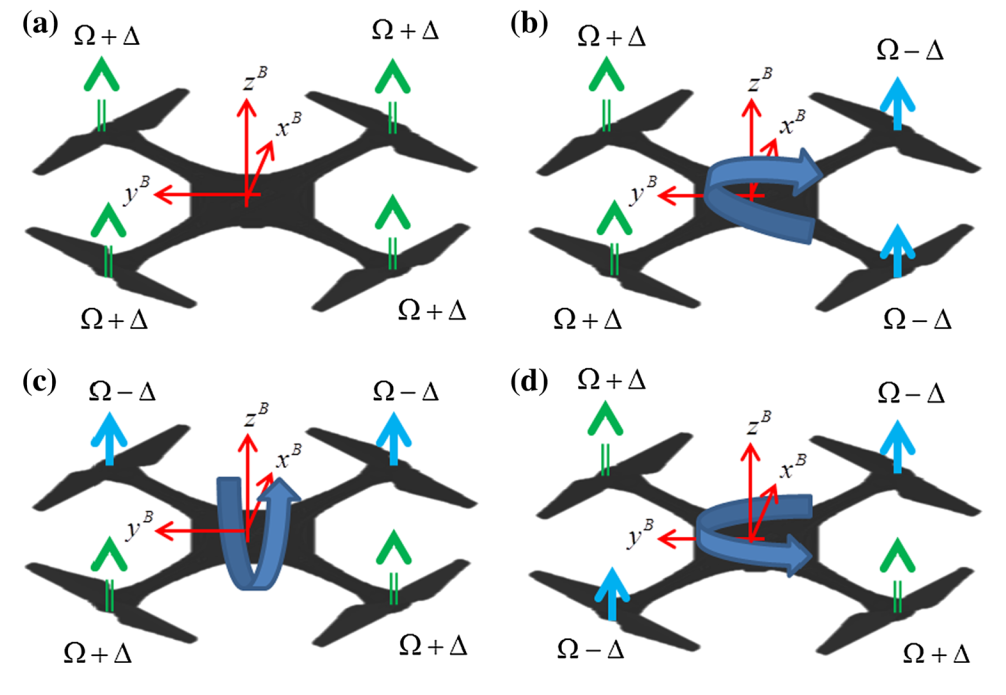
\includegraphics[scale=0.3]{partes/img/QUAV-modes.png}
    \caption[Modos de vuelo básicos de un QUAV.]{Modos de vuelo básicos de un QUAV \cite{multidrone2017review}. \textbf{(a)} Ascenso vertical, \textbf{(b)} \textit{Rolling}, \textbf{(c)} \textit{Pitching} y \textbf{(d)} \textit{Yawing}.} 
    \label{fig:QUAV-modes}
\end{figure}

\textit{Rolling} y \textit{Pitching} producen rotaciones sobre los ángulos \jim{\phi} y \jim{\theta} respectivamente, y producen una translación asociada en la dirección de los rotores que giran a menor velocidad \jim{\Omega - \Delta}. Efectivamente, \textit{Rolling} y \textit{Pitching} permiten mover al QUAV en la direcciones \jim{y_B} y \jim{x_B}. Por otro lado, \textit{Yawing} produce una rotación sobre el ángulo \jim{\psi} sin producir una translación asociada. \textit{Yawing} es importante porque es el modo de movimiento que modifica directamente el encabezamiento del QUAV.

\subsection{Localización GPS y coordenadas NED}

Tal como se menciona en la Sección \ref{sec:QUAV-sensors}, es habitual que un QUAV tenga acceso tanto a localización por visión como a localización por GPS, sin embargo, a efectos de este trabajo, se asume que el QUAV siempre utiliza localización por GPS. Para aplicaciones de evasion de obstáculos locales, utilizar directamente las coordenadas GPS puede resultar poco práctico debido a la diferencia de escalas. En concreto, la diferencia entre dos puntos cercanos en coordenadas GPS puede ser muy pequeña, lo que puede producir errores numéricos en el cálculo de la distancia entre dos puntos. Es por esto, que es importante establecer un sistema de coordenadas equivalente que no tenga este problema.

En el modelo geodésico del mundo WGS64, el que se utiliza en este trabajo, un punto en coordenadas GPS vienen dadas por la tupla latitud, longitud y altitud \jim{(\phi, \lambda, h)} \cite{2002convertGPS}. En la Figura \ref{fig:WGS64}, se muestra el elipsoide del modelo geodésico del mundo WGS64, donde se observa la coordenada \jim{(\phi, \lambda, h)} que representa el punto \jim{(x,y,z)}.

\begin{figure}[H]
    \centering
    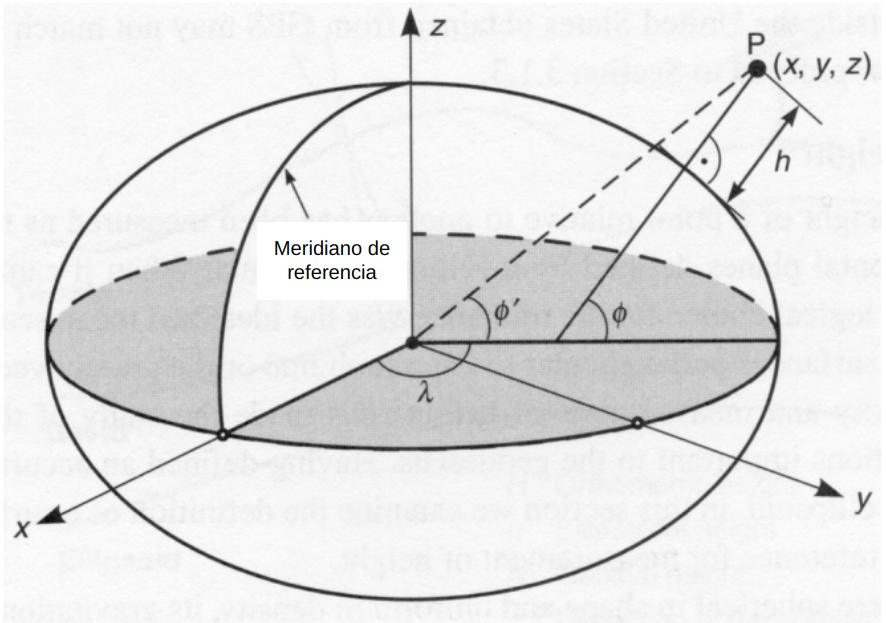
\includegraphics[scale=0.3]{partes/img/WGS64.png}
    \caption[Modelo geodésico del mundo WGS64.]{Modelo geodésico del mundo WGS64. Modificada de \cite{2002convertGPS}.} 
    \label{fig:WGS64}
\end{figure}

Dado \jim{S_{W}} el conjunto de puntos en la superficie del elipsoide WGS64. Un sistema de referencia sencillo de representar y que puede modelar los puntos \jim{(\phi, \lambda, h)} en el modelo WGS64, es el sistema de coordenadas NED (Norte, Este y Abajo; del inglés \textit{North, East, Down}) \cite{cai2011coordinate}. Este sistema es relativo a \jim{S_{W}} y sus puntos se representan con la tupla \jim{(n, e, d)} donde, dado un punto \jim{o = (\phi_0, \lambda_0) \in S_{W}}:

\begin{itemize}
    \item \jim{n} es el desplazamiento en metros hacia el \textbf{norte} del elipsoide a partir de \jim{o}.
    \item \jim{e} es el desplazamiento en metros hacia el \textbf{este} del elipsoide a partir de \jim{o}.
    \item \jim{h} es profundidad del punto en la \textbf{dirección normal} del elipsoide en \jim{o}.
\end{itemize}

El punto \jim{(\phi_0, \lambda_0, 0)} es el origen del sistema de coordenadas NED \cite{cai2011coordinate}, y suele definirse como el punto latitud, longitud de donde despega el QUAV \cite{multidrone2017review}.

Dada \jim{G: S_W \times S_W \longrightarrow \mathbb{R}^{+} \times \mathbb{R}^{+}} una función que recibe dos coordenadas \jim{a = (\phi_a, \lambda_a)} y \jim{b = (\phi_b, \lambda_b)} en \jim{S_W} y retorna el par real \jim{(\delta_n, \delta_e)} donde: 

\begin{itemize}
    \item \jim{\delta_n} es la longitud en metros del camino mas corto que va desde \jim{(\phi_a, \lambda_a)} hasta \jim{(\phi_b, \lambda_a)} sobre \jim{S_W}.
    \item \jim{\delta_e} es la longitud en metros del camino mas corto que va desde \jim{(\phi_a, \lambda_a)} hasta \jim{(\phi_a, \lambda_b)} sobre \jim{S_W}.
\end{itemize}

El Algoritmo \ref{alg:NED} muestra cómo transformar un punto \jim{(\phi, \lambda, h)} en WGS64 a NED.

\begin{algorithm}
\caption{Pseudo-código del algoritmo de transformación de coordenadas WGS64 a coordenadas NED}
\label{alg:NED}
\KwData{\jim{G}, \jim{(\phi, \lambda, h)}, \jim{(\phi_0, \lambda_0) \in S_{W}}}
\KwResult{\jim{(n, e, d)}}

$(\delta_n, \delta_e) = G((\phi_0, \lambda_0), (\phi, \lambda))$

$n = \text{sgn}(\phi - \phi_0) \cdot \delta_n$

$e = \text{sgn}(\lambda - \lambda_0) \cdot \delta_e$

$d = -h$;

\Return{\jim{(n, e, d)}}

\end{algorithm}


Donde \jim{\text{sgn}} es la función signo. \jim{G} usualmente es implementada utilizando la proyección de Mercator \cite{vis2018history} y existen una amplia selección de librerías de código abierto que la implementan.

\section{Visión estereoscópica}
\label{sec:teo-stereo}

El objetivo de los algoritmos de visión estereoscópica es obtener información tridimensional de una escena a partir de dos imágenes con distintas observaciones. Dado que la posición relativa entre las dos cámaras y los parámetros intrínsecos de cada una son conocidas, es posible obtener la información de profundidad de la escena utilizando relaciones geométricas entre las coordenadas tridimensionales y sus proyecciones en ambas imágenes \cite{sterovis}. Para que esto sea posible, es necesario que ambas imágenes estén rectificadas, esto es, que no tengan distorsión de lente y que se encuentren en el mismo plano; esto con el objetivo de que la diferencia entre una imagen y la otra sea un desplazamiento horizontal. La Figura \ref{fig:stereo-rectification} muestra un ejemplo del proceso de rectificación de un par de imágenes estéreo.

\begin{figure}[H]
    \centering
    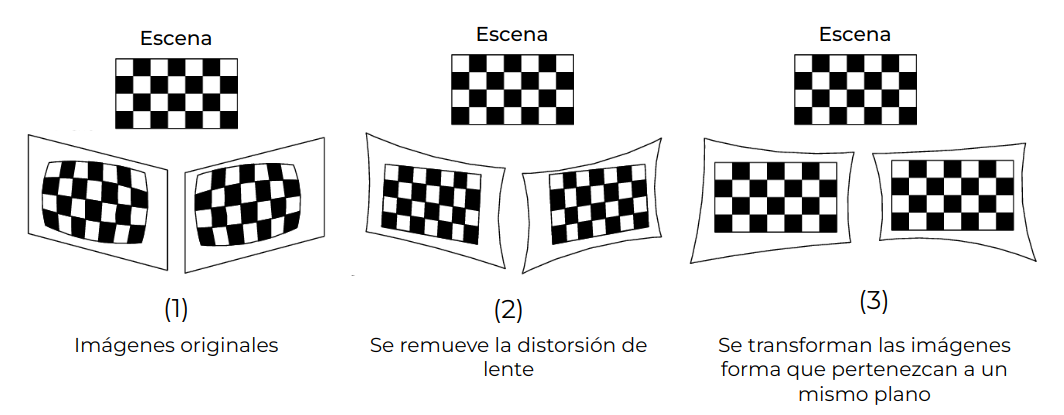
\includegraphics[scale=0.4]{partes/img/rectificacion.png}
    \caption[Ejemplo del proceso de rectificación de un par de imágenes estéreo.]{Ejemplo del proceso de rectificación de un par de imágenes estéreo. Modificada de \cite{Alberto2010}.}
    \label{fig:stereo-rectification}
\end{figure}

Con las imágenes rectificadas, el siguiente paso es obtener el desplazamiento horizontal entre las correspondencias píxel a píxel entre las dos imágenes, este desplazamiento se denomina disparidad. El arreglo bidimensional de la disparidad píxel a píxel entre dos imágenes estéreo se denomina mapa de disparidad, los mapas de disparidad nos permiten representar la información de la disparidad de todos los píxeles de una manera más accesible, ya que se puede interpretar como un imagen, tal como se muestra en la Figura \ref{fig:stereo-diparity-map}.

\begin{figure}[H]
    \centering
    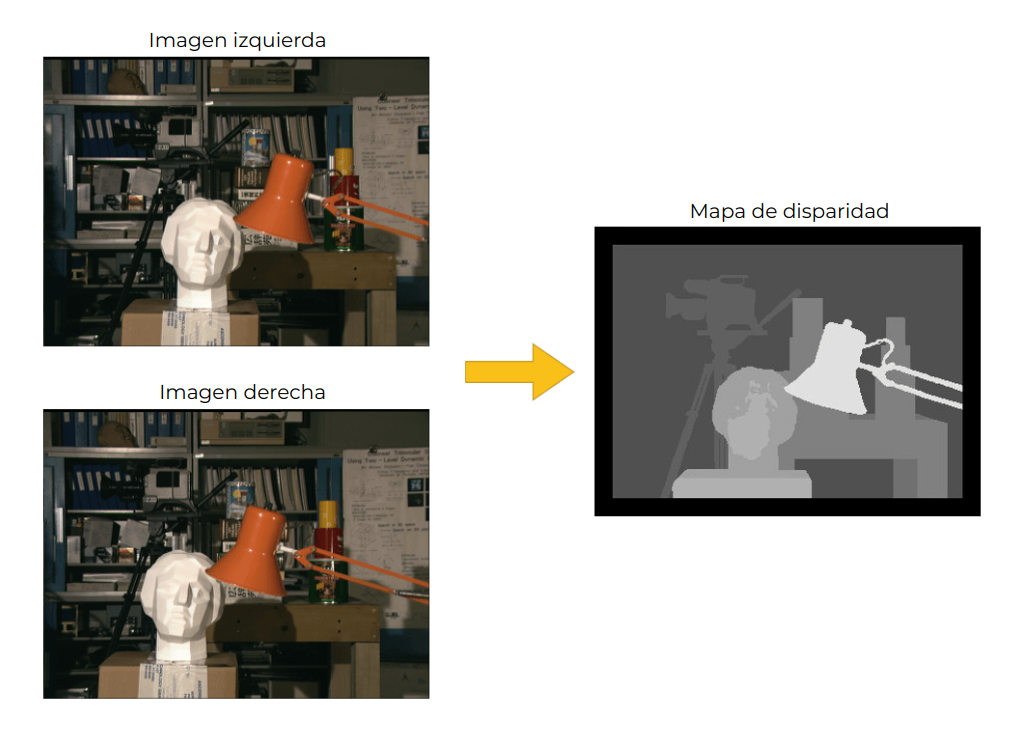
\includegraphics[scale=0.4]{partes/img/disparity-map.png}
    \caption[Ejemplo de la representación de un mapa de disparidad como una imagen.]{Ejemplo de la representación de un mapa de disparidad como una imagen\footnotemark.} 
    \label{fig:stereo-diparity-map}
\end{figure}
\footnotetext{Modificada de: \url{https://www.baeldung.com/cs/disparity-map-stereo-vision}}

Para calcular un mapa de disparidad hace falta establecer correspondencias píxel a píxel entre el par de imágenes estéreo. Un método para establecer estas correspondencias es el Emparejamiento de Bloques \cite{Baudes2009} (BM, del inglés \textit{Block Matching}). El BM consiste en obtener correspondencias entre imágenes estéreo rectificadas, tomando bloques de píxeles en la primera imagen y buscando los bloques mas similares en la segunda imagen; la búsqueda se realiza desplazando el dominio del bloque únicamente de forma horizontal a partir de la misma fila del bloque de la primera imagen; el criterio de búsqueda involucra una función de desemejanza entre bloques de píxeles, usualmente la Suma de Diferencias Absolutas (SAD, del inglés \textit{Sum of Absolute Differences}), y se seleccionan dos bloques como correspondientes si el valor de la función de desemejanza es mínimo local a lo largo de los posibles desplazamientos a partir de la posición inicial del bloque. En la Figura \ref{fig:stereo-block-matching} se ilustra un ejemplo de la correspondencia establecida por BM, y se observa el valor de la función de desemejanza en función de los desplazamientos (disparidad), el bloque seleccionado es aquel cuyo valor de la función de desemejanza sea mínimo local. BM permite obtener un valor de disparidad para cada píxel; finalmente, con este resultado se puede construir un mapa de disparidad.

\begin{figure}[H]
    \centering
    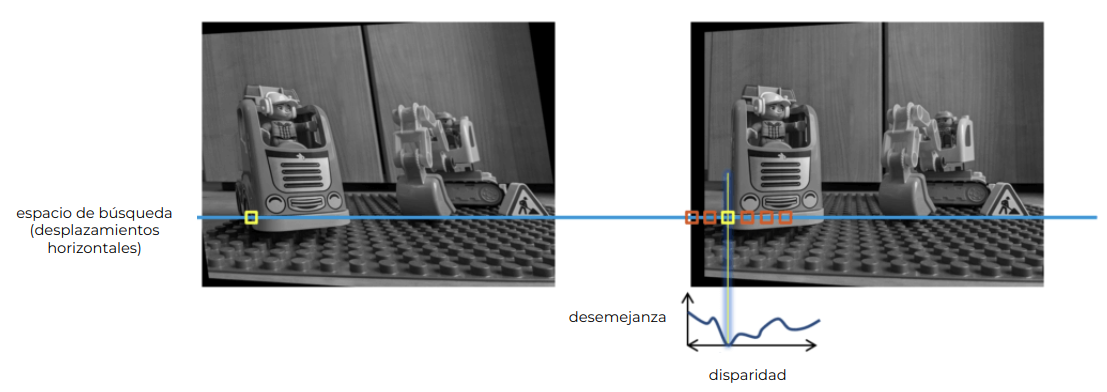
\includegraphics[scale=0.4]{partes/img/block-matching.png}
    \caption[Ejemplo del Emparejamiento de Bloques para establecer correspondencias entre un par de imágenes estéreo rectificadas.]{Ejemplo del Emparejamiento de Bloques para establecer correspondencias entre un par de imágenes estéreo rectificadas\footnotemark.} 
    \label{fig:stereo-block-matching}
\end{figure}
\footnotetext{Modificada de: \url{https://www.andreasjakl.com/understand-and-apply-stereo-rectification-for-depth-maps-part-2/}}

Una vez que se que se tiene el mapa de disparidad, es posible obtener la información de profundidad tridimensional de cada píxel utilizando relaciones geométricas, en particular, triangulación. En la Figura \ref{fig:stereo-triang} se muestra el modelo de un sistema de visión estereoscópica de dos cámaras paralelas \jim{C} y \jim{C^{\prime}}. En esta se observa: la distancia \jim{b}, que es la distancia entre las cámaras; la distancia \jim{f}, que es la distancia focal, es decir, la distancia entre el lente y el sensor; y un punto 3D en la escena, que corresponde al par de correspondencia píxel píxel \jim{u}, \jim{u^{\prime}} con disparidad \jim{d = (u_x - u^{\prime}_x)}. Los valores de \jim{b} y \jim{f} son determinados por el tipo y configuración de las cámaras, y se calculan mediante un proceso de calibración. Una vez conocidos, la profundidad \jim{D} del punto 3D en la escena con respecto al par estéreo se calcula utilizando la Ecuación \ref{eq:stereo-depth}. 

\begin{figure}[H]
    \centering
    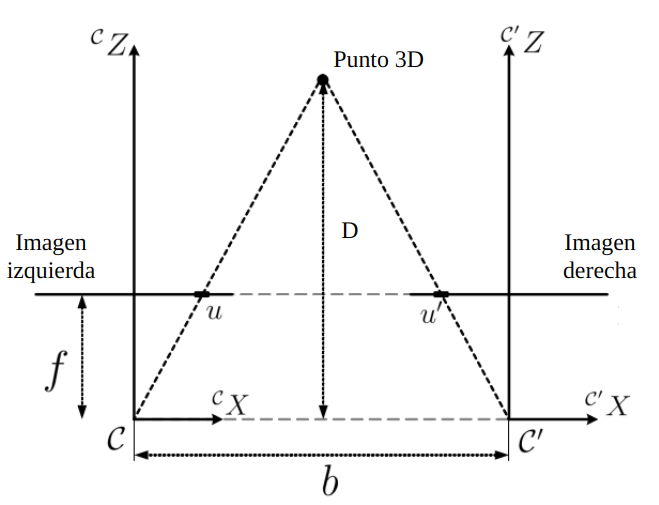
\includegraphics[scale=0.4]{partes/img/stereo-trangulation.png}
    \caption[Modelo de un sistema de visión estereoscópica de dos cámaras paralelas \jim{C} y \jim{C^{\prime}}.]{Modelo de un sistema de visión estereoscópica de dos cámaras paralelas \jim{C} y \jim{C^{\prime}}. Modificada de \cite{Alberto2010}.}
    \label{fig:stereo-triang}
\end{figure}

\begin{equation}
    \label{eq:stereo-depth}
    D =  \frac{f \cdot b}{u_x - u^{\prime}_x} = \frac{f \cdot b}{d}
\end{equation}

Si se calcula la profundidad \jim{D} para cada correspondencia representada en el mapa de disparidad se obtiene un mapa de profundidad que codifica la información tridimensional de la escena, dicho mapa de profundidad también se puede interpretar en una imagen de manera análoga a lo que se observa en la Figura \ref{fig:stereo-diparity-map}.

\section{Redes neuronales}
\label{sec:teo-neural}

Una red neuronal es un modelo matemático que trata de imitar el funcionamiento del cerebro humano para resolver problemas o tareas, donde las unidades básicas son las neuronas. Cada neurona recibe datos de entrada, realiza cálculos con ellos y produce una salida. La salida de una neurona se convierte en la entrada de otras neuronas, creando así una red de procesamiento. Tal como sus equivalentes biológicos, las redes neuronales son capaces de representar aprendizaje, así como adaptarse a través de la experiencia. Durante un proceso denominado entrenamiento, estas redes ajustan las conexiones entre sus neuronas, fortaleciendo o debilitando ciertas conexiones en función de la retroalimentación proporcionada por los datos observados. A medida que la red es expuesta a un mayor número de ejemplos y recibe retroalimentación constante, su capacidad para reconocer patrones, tomar decisiones o resolver problemas en esa tarea se fortalece.

Matemáticamente, una red neuronal es una serie de nodos interconectados, cada nodo recibe entradas de otros nodos y su respuesta se utiliza de entrada para otros nodos. Cada conexión tiene asociada un peso, que es un número real; cada nodo multiplica sus entradas con el respectivo peso de la conexión, suma los productos y le aplica una función de activación \cite{Gurney1997}; la función de activación es una función matemática simple que modela el proceso de disparo o activación de una neurona biológica. La Figura \ref{fig:nn-single-node} ilustra el funcionamiento de un nodo dentro de una red neuronal.

\begin{figure}[H]
    \centering
    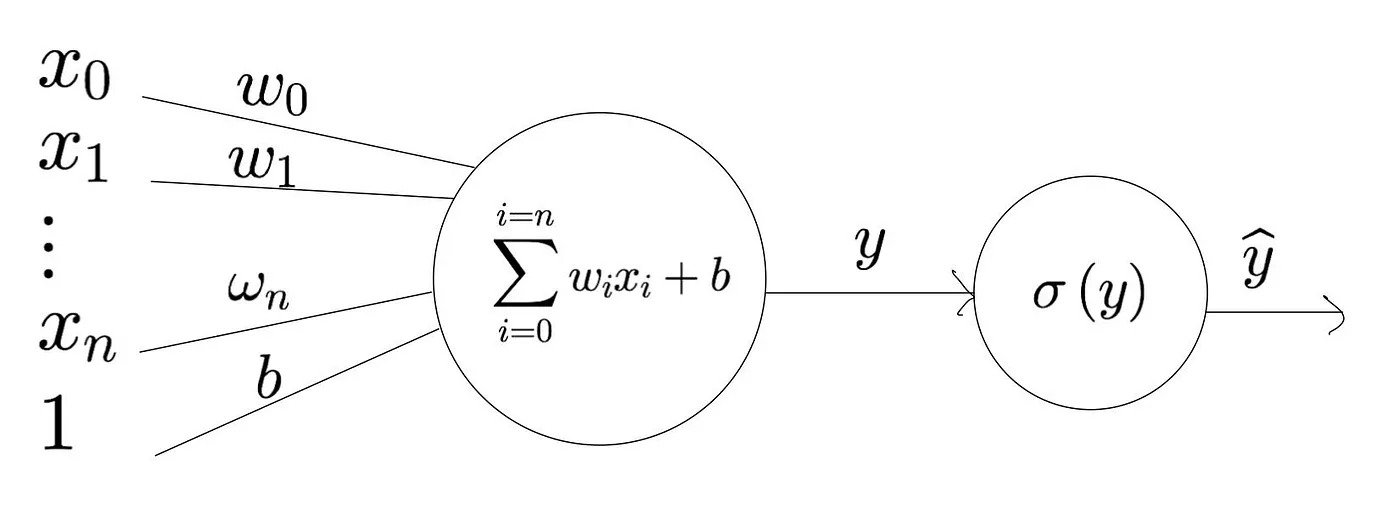
\includegraphics[scale=0.25]{partes/img/perceptron.jpg}
    \caption[Funcionamiento de un nodo de una red neuronal.]{
        Funcionamiento de un nodo de una red neuronal\footnotemark. \jim{n} es el número entradas del nodo. \jim{x_i} son las entradas del nodo y \jim{w_i} son los pesos asociados a sus conexiones, con \jim{0 \leq i \leq n}. Luego, \jim{\sigma} es la función de activación y \jim{b} es un peso asociado a una entrada constante, usualmente es llamado sesgo.
    } 
    \label{fig:nn-single-node}
\end{figure}
\footnotetext{Obtenida de: \url{https://medium.com/analytics-vidhya/perceptron-learning-from-discrete-to-continuous-02-b16ddf9e5ab6}}

La motivación matemática de la función de activación es introducir no linealidad a la salida del nodo, para ello existen una gama de funciones de activación ampliamente utilizadas, entre estas de encuentran: la función tangente hiperbólica, la función sigmoide y las Unidades Lineales Rectificadas (ReLU, del inglés \textit{Rectified Linear Units}), la Ecuación \ref{eq:tanh}, la Ecuación \ref{eq:sigmoid} y la Ecuación \ref{eq:relu} respectivamente muestran las definiciones de las funciones mencionadas anteriormente.

\begin{equation}
    \label{eq:tanh}
    \tanh(x) = \frac{\sinh(x)}{\cosh(x)} = \frac{e^x - e^{-x}}{e^x + e^{-x}}
\end{equation}

\begin{equation}
    \label{eq:sigmoid}
    \sigma(x) = \frac{1}{1 + e^{-x}}
\end{equation}

\begin{equation}
    \label{eq:relu}
    \mathrm{ReLU}(x)= \begin{cases} 
        0 & \text { si } x<0 \\
        x & \text { si } x \geq 0
    \end{cases}
\end{equation}

Las redes neuronales se pueden estructurar por capas, cada capa tiene una serie de nodos que reciben sus entradas de todos los nodos de la capa anterior y a su vez sirven de entrada todos los nodos de la capa superior; no existen conexiones entre nodos que pertenezcan a una misma capa y no existen capas que reciban como entrada a los nodos de alguna capa superior. Cuando una red neuronal se estructura por capas de la forma descrita anteriormente se le denomina Red Neuronal de Alimentación hacia adelante \cite{huang2019deep}, FFNN del inglés \textit{Feed-forward Neural Network}. 

\begin{figure}[H]
    \centering
    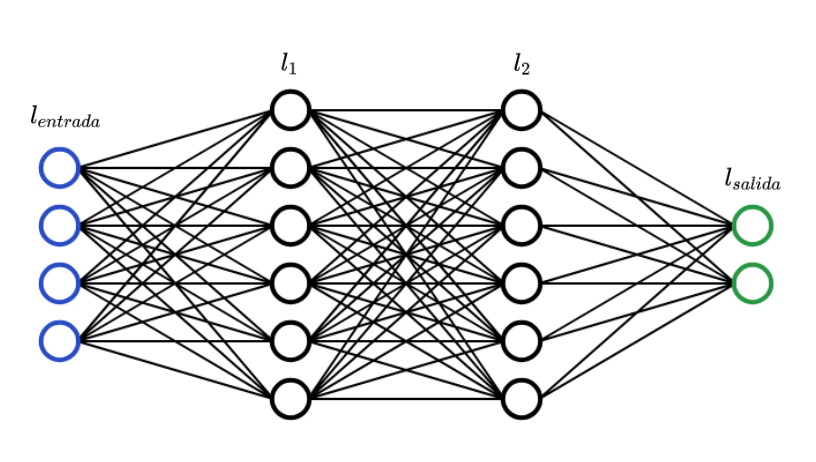
\includegraphics[scale=0.4]{partes/img/nn-capas.png}
    \caption[Ejemplo de una FFNN con dos capas ocultas.]{
        Ejemplo de una FFNN con dos capas ocultas\footnotemark. \jim{l_{entrada}} y \jim{l_{salida}} son las capas de entrada y de salida respectivamente. \jim{l_1} y \jim{l_2} son las capas ocultas, también llamadas capas completamente conectadas, FC del inglés \textit{Fully Connected}.
    } 
    \label{fig:nn-layers}
\end{figure}
\footnotetext{Modificada de: \url{https://victorzhou.com/series/neural-networks-from-scratch/}}


Un ejemplo de una FFNN de muestra en la Figura \ref{fig:nn-layers}. Las FFNN tienen una capa de entrada y una de salida (\jim{l_{entrada}} y \jim{l_{salida}} en la Figura \ref{fig:nn-layers}), la capa de entrada recibe el estimulo inicial de la red, mientras que la capa de salida retorna la respuesta de la red al estímulo. Además, las FFNN se caracterizan por el número de capas FC (\jim{l_1} y \jim{l_2} en la Figura \ref{fig:nn-layers}), mientras más capas ocultas, se dice que la red es más ``profunda". El conjunto de los pesos de los nodos de una red se denomina \jim{\theta}, mientras que un peso en particular se denomina \jim{w_{j}} donde \jim{j} es el índice de la transición asociada al peso. Al modificar pesos \jim{\theta} se modifica el comportamiento de la red ante un estimulo; diferentes combinaciones de valores de \jim{\theta} producen comportamientos distintos; así, la representación del ``conocimiento" de una red neuronal se encuentra almacenado en sus pesos \jim{\theta}. Mediante algoritmos de aprendizaje automático se pueden modificar sistemáticamente los pesos de la red neuronal para que se adapte a una tarea en especifica, este proceso de adaptación también es denominado entrenamiento \cite{Gurney1997}.

\subsection{Retro-propagación}

El algoritmo de retro-propagación (del inglés \textit{backpropagation}) es un algoritmo de aprendizaje supervisado que se utiliza para entrenar redes neuronales. Este algoritmo ajusta los pesos de las conexiones entre los nodos de la red neuronal de manera que la red pueda realizar una tarea en específico (clasificación o regresión por ejemplo). El algoritmo de retro-propagación utiliza el denominado descenso de gradiente (del inglés \textit{Gradient Descent}), el cual es un método utilizado para minimizar una función de pérdida que cuantifica el error entre las predicciones de la red y los valores objetivos asociados a la tarea seleccionada.

\subsubsection*{Descenso de gradiente}

El aprendizaje automático supervisado presenta iterativamente un conjunto de patrones de entrada (\jim{X}) y de salida (\jim{Y}) al modelo, en este caso una red neuronal. En cada iteración se modifican los pesos \jim{\theta} de acuerdo a una regla de actualización cuyo objetivo es que la salida de la red se asemeje a la salida deseada \cite{Gurney1997}. Para realizar estos cambios, la regla de actualización debe cuantificar que tan bien la red neuronal modela los datos que se le presentan; es por esto que se define una función de costo o error \textit{E} que dado un dado de entrada \jim{x_k}, el vector deseado \jim{y_k} y los pesos \jim{\theta} de la red, retorna \jim{E(x_k, y_k, \theta)} que cuantifica que tan similar a \jim{y_k} es la salida de la red (parametrizada por \jim{\theta}) cuando se le pasa como entrada \jim{x_k}. El objetivo es que la red sea capaz de modelar la relación entre los patrones de entrada \jim{X} y salida \jim{Y}, en otras palabras, se quiere minimizar la función descrita en la Ecuación \ref{eq:loss}; esta función se denomina función de pérdida, donde \jim{|X| = |Y|} y \jim{x_k, y_k} son el patrón entrada salida número \jim{k} con \jim{x_k \in X \wedge y_k \in Y}. Finalmente el problema de minimización tratado en este trabajo es el descrito en la Ecuación \ref{eq:optim-problem}.

\begin{equation}
    \label{eq:loss}
    L(X, Y, \theta) = \sum_{k = 1}^{|X|} E(x_k, y_k, \theta)
\end{equation}

\begin{equation}
    \label{eq:optim-problem}
    \min_{\theta} L(X, Y, \theta)
\end{equation}

Tal como su nombre lo indica, el descenso de gradiente en cada iteración se mueve en la dirección del gradiente, esto lo hace siguiendo la regla de actualización:

\begin{equation}
    \label{eq:gd-update-rule}
    \theta = \theta - \alpha \nabla_{\theta} L(X, Y, \theta)
\end{equation}

Donde \jim{0 < \alpha < 1} es un número real llamado "tasa de aprendizaje"; \jim{\alpha} se encarga de que la regla de actualización no produzca cambios drásticos que puedan dificultar la convergencia del algoritmo. Luego, la regla de actualización de cada peso individual \jim{w_{j}} viene dada por:

\begin{equation}
    \label{eq:gd-update-rule-item}
    w_{j} = w_{j} - \alpha \frac{\partial L(X, Y, \theta)}{\partial w_{j}}
\end{equation}

Estas regla de actualización se aplica iterativamente sobre el conjunto de patrones entrada salida (también llamado conjunto de entrenamiento) hasta alcanzar un criterio de convergencia, como un valor umbral de la función de pérdida o un número de iteraciones. Justamente esta es la descripción del algoritmo del descenso de gradiente.

Dado un conjunto de datos de entrada \jim{X}, un conjunto de valores deseados \jim{Y}, la tasa de aprendizaje \jim{\alpha} y una función booleana \jim{Q(\theta)} que sirve como criterio de convergencia. El Algoritmo \ref{alg:dg} muestra el pseudo-código del proceso de retro-propagación usando descenso de gradiente.

\begin{algorithm}
\caption{Pseudo-código del algoritmo de retro-propagación usando descenso de gradiente}
\label{alg:dg}
\KwData{\jim{X, Y, \alpha, Q}}
\KwResult{\jim{\theta}}

Inicializar los pesos \jim{\theta} en ceros o en valores aleatorios cercanos a cero

\While{\jim{\neg Q(\theta)}}{
    \For{\jim{w_j \in \theta}}{
        \jim{w_{j} = w_{j} - \alpha \frac{\partial L(X, Y, \theta)}{\partial w_{j}}}
    }
}
\end{algorithm}

\subsubsection*{Sub-ajuste y sobre-ajuste}

La arquitectura de una red neuronal (número de capas y de nodos por capa) y el criterio de convergencia del descenso de gradiente deben elegirse cuidadosamente para evitar sesgos que puedan afectar negativamente el rendimiento del modelo. Hay dos tipos de errores a los que puede conducir un sesgo inapropiado: sub-ajuste y sobre-ajuste. El sub-ajuste (del inglés \textit{underfitting}) ocurre cuando la arquitectura de la red es demasiado simple para representar la relación entre los datos de entrada y los valores deseados del conjunto de entrenamiento, o cuando el criterio de convergencia es demasiado temprano. Por otro lado, el sobre-ajuste (del inglés \textit{overfitting}) ocurre cuando la arquitectura de la red es muy compleja o se realizan demasiadas iteraciones del descenso de gradiente, lo que hace que el modelo se ajuste demasiado al conjunto de datos de entrenamiento. Los modelos con sub-ajuste o sobre-ajuste no generalizan correctamente y, por lo tanto, no sera buenos al momento de realizar inferencia sobre datos que estén más allá de lo que se observó durante el entrenamiento.

\subsection{Redes neuronales convolucionales}

Cuando se desea utilizar una imagen como entrada de una red neuronal, cada píxel de la imagen es una entrada de la red; considerando que incluso imágenes de resoluciones relativamente bajas contienen un número de píxeles en el orden de los miles y hasta tres canales de color, si se utilizara una red con solo capas FC, la cantidad de pesos a entrenar sería muy elevada debido a la alta cantidad de entradas; una imagen a color de 300 píxeles de ancho por 300 de alto necesitaría \jim{300 \cdot 300 \cdot 3 = 270000} nodos de entrada, colocando el número de pesos de la red en el orden los cien miles con tan solo una capa, por esto el uso de redes neuronales con solo capas FC no es conveniente para trabajar con imágenes.

Las redes neuronales convolucionales (CNN, del inglés \textit{Convolutional Neural Networks}) son un tipo de red neuronal FFNN, principalmente utilizadas para el procesamiento digital de imágenes, que debido a su estructura permiten reducir la cantidad de pesos necesarios a entrenar; habilitando un proceso de entrenamiento más sencillo y a mayor velocidad \cite{Lecun2010}. Las CNN incorporan tres tipos de capas: las capas convolucionales, las capas de submuestreo (del inglés \textit{pooling layers}) y capas FC generalmente al final de la red.

Las CNN suelen componerse de dos partes: un denominado extractor de características, conformado por capas convolucionales y capas de submuestreo; y parte FC cuyo objetivo varia dependiendo de la tarea que se requiere de la red (regresión o clasificación por ejemplo). En la Figura \ref{fig:cnn-sample} se muestra un ejemplo de la arquitectura de una CNN.

\begin{figure}[H]
    \centering
    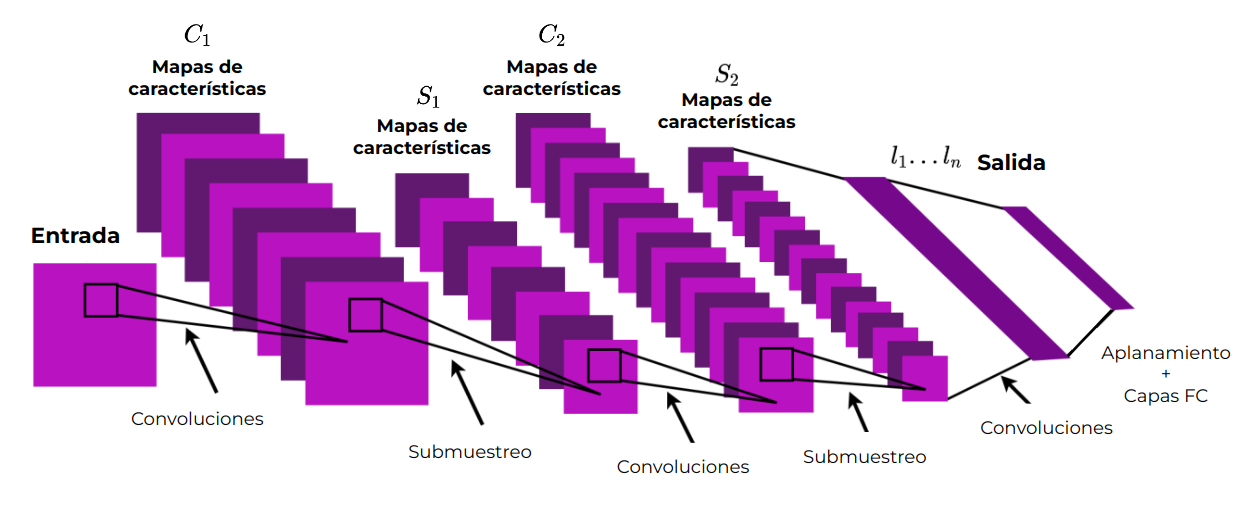
\includegraphics[scale=0.35]{partes/img/CNN-sample.png}
    \caption[Ejemplo de la arquitectura de una CNN.]{
        Ejemplo de la arquitectura de una CNN \cite{Lecun2010}. \jim{C_1} y \jim{C_2} son los resultados de capas convolucionales, \jim{S_1} y \jim{S_2} son los resultados de capas de submuestreo. \jim{l_1 ... l_n} son \jim{n} capas FC. Entre \jim{S_2} y \jim{l_1} se realiza un proceso de aplanamiento, que concatena los mapas de características de \jim{S_2} para producir un vector de características que sirve de entrada para \jim{l_1}.
    } 
    \label{fig:cnn-sample}
\end{figure}

La intuición detrás de las capas convolucionales es la de la aplicación de filtros en espacio sobre imágenes para la extracción de mapas que codifican información de la entrada \cite{Gupta2013} \cite{Coady2019}. Las capas convolucionales realizan operaciones de convolución discreta a la matriz (imagen) de entrada, utilizando filtros también llamados \textit{kernels}. El resultado de una capa convolucional es una matriz en donde cada componente corresponde a la multiplicar uno de los \textit{kernels} con una región de la imagen de entrada, sumar los resultados y opcionalmente aplicar una función de activación. Estas capas de usan para la detección de características, es por eso que a la salida de estas capas se le da el nombre de ``mapa de características". El ancho y el alto de este mapa dependen de las dimensiones del \textit{kernel}, mientras que su número de canales es igual al número de \textit{kernels} utilizados por la capa.

Las capas de submuestreo se tienen la finalidad de filtrar características poco relevantes de la entrada, su salida es un mapa de características donde cada componente es el resultado de una operación de reducción de dimensionalidad de una región del mapa de entrada. La operación de reducción de dimensionalidad usualmente es de uno de los siguientes tipos: promedio de la región seleccionada, en cuyo caso se le llama submuestreo por promedio (del inglés \textit{average pooling}); o máximo de la región seleccionada, llamando entonces submuestreo por máximo (del inglés \textit{max pooling}). El efecto de reducción de dimensionalidad ayuda a reducir el número de operaciones convolucionales de capas posteriores, haciendo el proceso de entrenamiento mas sencillo y veloz.

Entre el extractor de características y la parte FC se hace un proceso de aplanamiento (del inglés \textit{flattening}), cuyo resultado es la concatenación de los mapas de características para producir un vector de características que sirve de entrada para las capas FC de la red. La sección FC recibe el vector de características y genera una salida cuyas dimensiones dependen de la tarea en la cual se esta entrenando la red, estas capas FC siguen la misma estructura descrita en la Sección \ref{sec:teo-neural}.

\section{Comunicación entre procesos}
\label{sec:teo-interprocess}

La comunicación entre procesos, comúnmente abreviada como IPC (por sus siglas en inglés, Inter-Process Communication), se refiere al conjunto de técnicas y mecanismos utilizados para permitir que diferentes procesos intercambien información entre sí de forma asíncrona. Esta comunicación es fundamental en escenarios donde varias aplicaciones deben colaborar para lograr una funcionalidad más amplia. A través de IPC, los procesos pueden compartir datos, sincronizar su ejecución, coordinar tareas y garantizar la seguridad y eficiencia en la gestión de recursos compartidos. Algunos de los métodos de IPC utilizados comúnmente son las tuberías (del inglés \textit{pipes}), los \textit{sockets} y la memoria compartida \cite{IPCEval2015}.

\subsection*{Tuberías}

Una tubería o \textit{pipe} es un método de comunicación unidireccional que permite la transferencia serial de información desde el proceso escritor al proceso lector. La capacidad de transferencia de datos de un tubería esta limitada por un búfer de tipo primero que entra, primero que sale (FIFO, del inglés \textit{First In, First Out}); cuando el escritor envía datos estos se agregan al búfer, de forma análoga cuando el lector procesa datos estos se eliminan del búfer; si el escritor escribe más rápido de lo que el lector consume datos y si el búfer de la tubería está lleno, el escritor se bloqueará hasta que haya más capacidad disponible. De manera similar, si el lector lee cuando la tubería está vacía, el lector se bloqueará \cite{IPCEval2015}. Con una tubería se pueden implementar esquemas de comunicación de mayor nivel de tipo productor-procesador (Pub/Sub, del inglés \textit{Publisher/Subscriber}) siempre y cuando solo exista solo un productor y solo un procesador.

\subsection*{\textit{Sockets}}

Un \textit{socket} es un mecanismo de comunicación bidireccional que se puede utilizar para comunicar un proceso con otro proceso, bien sea dentro de la misma máquina o en una máquina diferente \cite{IPCEval2015}. Los datos enviados a través de un \textit{socket} se dividen en fragmentos llamados paquetes. Un protocolo, como TCP/IP, especifica cómo se transmiten estos paquetes a través del \textit{socket}. Un \textit{socket} se identifica de manera única mediante una combinación de la dirección IP de la máquina y un número de puerto. La bidireccionalidad de los \textit{sockets} permite construir esquemas de comunicación a alto nivel sin restricciones de cardinalidad (tales como Pub/Sub con muchos productores y muchos receptores), si bien la implementación de estos esquemas puede ser complicado,  existen múltiples librerías de implementaciones estables de estos, tales como ZeroMQ \cite{zeroMQ}.

\subsection*{Memoria compartida}

La memoria compartida permite a dos o más procesos acceder al mismo espacio de memoria, este espacio es mapeado al espacio de direcciones de memoria de cada uno de los procesos participantes \cite{IPCEval2015}. Dado que esta comunicación es similar a cualquier otra referencia de memoria, no implica ninguna llamada al sistema ni latencias inducidas por protocolos. Por lo tanto, generalmente la memoria compartida ofrece latencias muy bajas. Sin embargo, el sistema no proporciona ningún mecanismo sincronización implícito para los accesos a la memoria compartida; esto significa que el uso descuidado de la memoria compartida puede producir condiciones de carrera \cite{IPCEval2015}. El uso de mecanismos de primitivas como los semáforos o los \textit{mutex} pueden habilitar el uso de la memoria compartida sin riesgo de inconsistencia en los datos, pero su implementación es responsabilidad del programador.

\section{Resumen}

En este capítulo se establecen las bases teóricas necesarias para el desarrollo del trabajo, incluyendo el modelado de vehículos aéreos no tripulados de cuatro rotores y el procedimiento para la obtención de mapas de profundidad a partir de un sistema de cámaras estereoscópicas. Adicionalmente, se explican los fundamentos de las redes neuronales, su proceso de entrenamiento y sus variantes enfocadas al procesamiento de imágenes, las CNN. Finalmente, se describieron algunos métodos de comunicación entre procesos que nos serán útiles durante el desarrollo del presente trabajo.

En el siguiente capítulo, se hace una revisión del estado del arte de los métodos de evasión de obstáculos para drones y se profundiza en \textit{Learning high-speed flight in the wild}, un método bastante atractivo para el desarrollo de este trabajo en el contexto de la plataforma disponible para su implementación.